%\documentclass[14pt, notes]{beamer}
\documentclass[14pt]{beamer}

%\usepackage{pgfpages}
%\setbeameroption{show notes}
%\setbeameroption{show notes on second screen=right}

%encoding
\usepackage[utf8]{inputenc}

%language
\usepackage[russian]{babel}
\usepackage{amsmath}
\usepackage{bm}
\usepackage{graphicx}
\usepackage{hyperref}
\usepackage{setspace}
\usepackage{tikz}
\usepackage{adjustbox}
\usepackage{marvosym}
\usepackage{animate}
\usetikzlibrary{shapes,arrows,positioning}
\makeatletter
%\@ifundefined{verbatim@out}{\newwrite\verbatim@out}{}
\makeatother
\graphicspath{{images/}}%путь к рисункам

\usepackage{tikz}
\usetikzlibrary{shapes,arrows}

\tikzstyle{decision} = [diamond, draw, fill=blue!20, text width=4.5em, text badly centered, node distance=3cm, inner sep=0pt]
\tikzstyle{block} = [rectangle, draw, fill=blue!20, text width=11em, text centered, rounded corners, minimum height=2em]
\tikzstyle{line} = [draw, -latex    ]
\tikzstyle{cloud} = [draw, ellipse,fill=red!20, node distance=3cm, minimum height=2em]

\setbeamerfont{author in head/foot}{size=\small}
\setbeamerfont{title in head/foot}{size=\footnotesize}
\setbeamercovered{invisible}
\setbeamertemplate{navigation symbols}{}%remove navigation symbols

\title[Моделирование клапанов]{Математическое моделирование работы искусственного сердечного клапана}
\date{\today}
\author[Долгов Д.А.]{Долгов Д.А.}
\institute{Кемеровский Государственный Университет \\
    \vspace{0.7cm}
    \vspace{0.7cm}
} 
\usetheme[numbers, totalnumbers, minimal, nologo]{Statmod}
% Привычный шрифт для математических формул
\usefonttheme[onlymath]{serif}

\definecolor{statmodblue}{RGB}{100,10,30}
\definecolor{statmodsand}{RGB}{244,215,103}

\begin{document}
\maketitle

%description of the problem
\begin{frame}
\frametitle{Введение}
Искусственные сердечные клапаны являются одними из самых сложных медицинских
устройств, используемых в кардиохирургии. Требования к функционированию
клапанов очень велики - необходимо, чтобы он минимизировал турбулентность,
создавал небольшой объем регургитации, позволял избегать зон застоя, разделения
потока и т.д.
\end{frame}
\note{
    объем регургитации - объем обратного течения (из желудочка в атриум)
}

\begin{frame}
\frametitle{Обзор исследований}
Работы, в которых расматривается только клапан и его деформации, моделируя
поток в упрощенном виде или получая данные о давлении экспериментально. См. например:\\
\par
{\tiny
    \begin{itemize}
        \item[\MVRightarrow] Бокерия Л.А., Скопин И.И., Сазоненков М.А., Тумаев Е.Н., Механическое напряжение в створках митрального клапана и биопротеза в митральной позиции. Влияние геометрии фиброзного кольца на величину напряжения створок/Клиническая физиология кровообращения, 2008, №2
        \item[\MVRightarrow] Сазоненков, М.А. Расчет напряжений в структурах нормального митрального клапана. / М.А. Сазоненков, Е.Н. Тумаев, И.И. Скопин // Бюллетень НЦ ССХ им. А.Н. Бакулева РАМН. Сердечно-сосудистые заболевания. Четырнадцатый Всероссийский съезд сердечно-сосудистых хирургов. – 2008. - Т 9, N 6. - с. 55.
        \item[\MVRightarrow] Kunzelman K.S., Reimink M.S. et al  Annular dilatation increases stress in the mitral valve and delays coaptation: a finite element computer model. (1997) Cardiovasc Surg 5(4):427–434
        \item[\MVRightarrow] Weinberg E. Dynamic simulation of heart mitral valve with transversely isotropic material model. Massachusetts Institute of Technology (2005)
        \item[\MVRightarrow] Kim H.S. Nonlinear multi-scale anisotropic material and structural models for prosthetic and native aortic heart valves. Georgia Institute of Technology (2009)
    \end{itemize}
}
\end{frame}
\note{
Отметить, что рассматриваются работы, посвященные именно математическому моделированию клапанов,
а не экспериментальному. На эту тему мало русскоязычных работ - даже в монографии "Искусственные клапаны сердца"
(Орловский, Гриценко, Юхнев, Евдокимов, Гавриленков),
где описан крупный вклад отечественных ученых в области клапанов, в разделе "Математическое моделирование" нет
упоминаний о русскоязычных работах.
Существует достаточно много (по крайней мере, зарубежных) исследований,
посвященных математическому моделированию сердечных клапанов. В ранних моделируются
только достаточно простые клапаны (по структуре, двумерные и проч.).
Существует много современных работ, которые изучают клапан только с точки зрения
эластичности, напряжений, возникающих при деформации и проч (при этом данные о давлении жидкости
берутся либо из эксперимента, либо упрощенные, например течение Пуазеля).
Самый перспективный вид исследований те, которые полноценно описывают взаимодействие потока и клапана,
т.е. IBM
}

\begin{frame}
\frametitle{Обзор исследований}
Исследования, которые рассматривают полноценное взаимодействие
''жидкость-клапан'', зачастую относятся к методу погруженной границы, т.к. он
позволяет считать клапан сколь угодно тонким:
\par
{\tiny
    \begin{itemize}
        \item[\MVRightarrow] Орловский П.И., Гриценко В.В., Юхнев А.Д., Евдокимов С.В., Гавриленков В.И. Искусственные клапаны сердца. СПб. 2007. - 448с
        \item[\MVRightarrow] Peskin, Charles S. "Numerical analysis of blood flow in the heart." Journal of computational physics 25.3 (1977): 220-252.
        \item[\MVRightarrow] Luo, X. Y., et al. "Effect of bending rigidity in a dynamic model of a polyurethane prosthetic mitral valve." Biomechanics and modeling in mechanobiology 11.6 (2012): 815-827.
        \item[\MVRightarrow] Flamini, Vittoria, Abe DeAnda, and Boyce E. Griffith. "Immersed boundary-finite element model of fluid-structure interaction in the aortic root." (2015).
    \end{itemize}
}
\end{frame}

% valves placement
\begin{frame}
\frametitle{Схема расположения клапанов}
    \begin{center}
        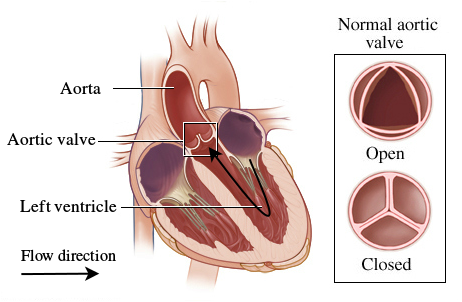
\includegraphics[width=8.5cm]{aorta_scheme.png}
    \end{center}
\end{frame}

% blood structure scheme
\begin{frame}
\frametitle{Схема структуры крови}
    \begin{center}
        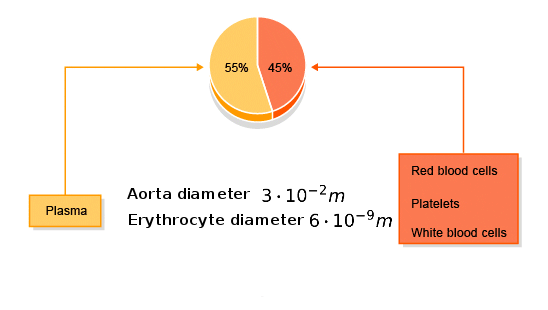
\includegraphics[width=8.5cm]{blood_scheme3.png}
    \end{center}
\end{frame}

\begin{frame}
\frametitle{Искусственный клапан}
    \begin{center}
        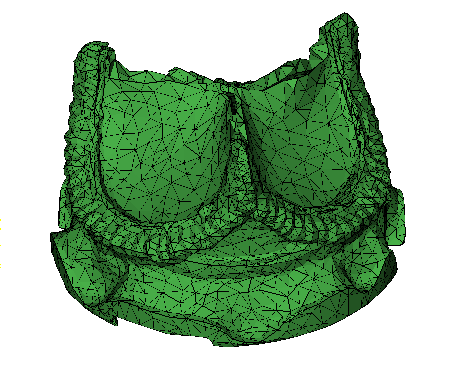
\includegraphics[width=6cm]{real_valve_3_1.png}
        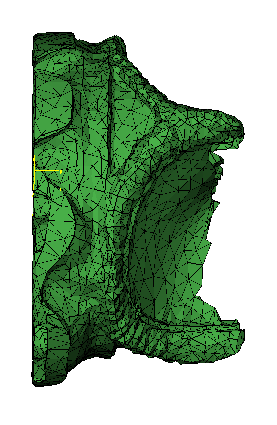
\includegraphics[width=3cm]{real_valve2_1.png}
    \end{center}
\end{frame}

\begin{frame}
\frametitle{Описание модели}
Рассмотрим задачу о течении крови внутри крупных сосудов с клапаном. Кровь
является неоднородной и состоит из плазмы и взвешенных в ней форменных
элементов. Клапан является гибким и изменяет свою форму под воздействием
течения.

Будем моделировать кровь как вязкую, несжимаемую двухкомпонентную
жидкость, створки клапана - как непроницаемую поверхность заданной формы,
обладающую определенной жесткостью.
\end{frame}

%description of the problem: schema
\begin{frame}
\frametitle{Описание модели}
    \begin{center}
        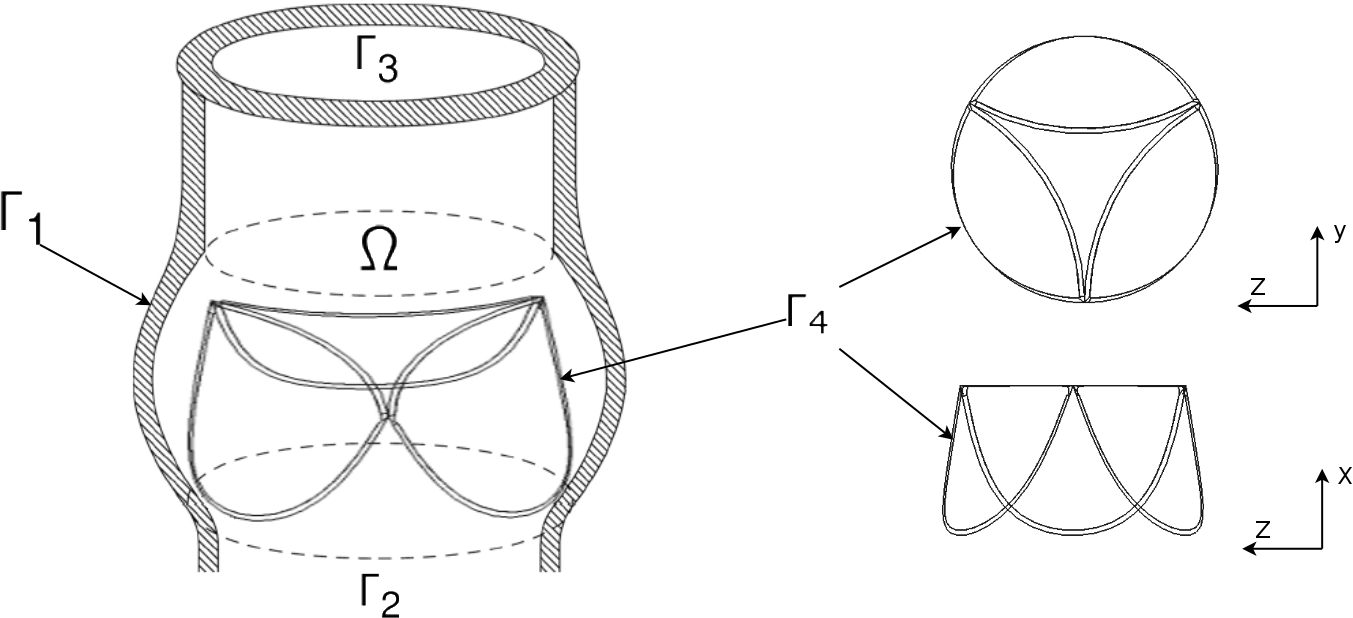
\includegraphics[width=11cm]{aorta_valve_scheme.png}
    \end{center}
\end{frame}
\note{$\Gamma_1$ - гибкие стенки, $\Gamma_2,\Gamma_3$ - вход/выход}

% navier stokes equations
\begin{frame}
\frametitle{Моделирование течения}
Система уравнений Навье-Стокса:
\begin{gather}
    \label{eq:motion}
    \frac{\partial u}{\partial t} + (u \cdot \nabla) u = - \frac{1}{\rho} \nabla p + \nabla \cdot \sigma + f\\
    \label{eq:continuity}
    \frac{\partial \rho}{\partial t} + \nabla \cdot (\rho u) = 0 
\end{gather}
где $\sigma = \mu (\nabla u + (\nabla u)^{T})$, $\bar{x} = (x, y, z) \in \Omega$ с начальными и краевыми условиями
\begin{gather*}
    u(\bar{x}, t_0) = u_0;\ \frac{\partial u}{\partial n}|_{\Gamma_2, \Gamma_3} = 0\\
    p|_{\Gamma_2} = p_{in};\ p|_{\Gamma_3} = p_{out} \\
\end{gather*}

\end{frame}
\note{Уравнения записаны в векторном виде, $\sigma$ - вязкий тензор напряжений}

% concentration
\begin{frame}
\frametitle{Концентрация}
Уравнение для расчета концентрации примеси в жидкости:
\begin{gather}
    \label{eq:concentration}
    \frac{\partial c}{\partial t} + u \cdot \nabla c = 0
\end{gather}
с начальными и краевыми условиями
\begin{gather*}
    c(\bar{x}, 0) = c_0(\bar{x})\\
    c(\bar{x}, t)|_{\Gamma_2} = c_s(\bar{x}, t)
\end{gather*}

\end{frame}

% concentration: dependencies
\begin{frame}
\frametitle{Концентрация}
Плотность и вязкость зависят от концентрации:
\begin{gather}
    \label{eq:concentration_viscosity}
    \mu = c (\mu_2 - \mu_1) + \mu_1\\
    \label{eq:concentration_density}
    \rho = c (\rho_2 - \rho_1) + \rho_1
\end{gather}

где $\mu_1, \mu_2, \rho_1, \rho_2$ - вязкости и плотности обоих компонент.
\end{frame}

% boundary
\begin{frame}
\frametitle{Сопротивление деформации}
В каждой точке сосуда и клапана определена поверхностная сила, которая стремится вернуть систему в равновесное положение
\begin{gather}
    \label{eq:strain_energy}
    F =  \frac{\partial}{\partial s}(T \tau) + \frac{\partial^2}{\partial s^2} \Big( E \cdot I \frac{\partial^2}{\partial s^2} X \Big)
\end{gather}
\begin{gather}
    \label{eq:define_boundary_force}
    F = k \cdot \|X - X_0\|
\end{gather}
\end{frame}
\note{$E$ - модуль Юнга, $I$ - момент инерции поперечного сечения, $T$ - напряжение фибры, $\tau$ - единичный тангенциальный вектор, касательный к фибре.}

% solve method 
\begin{frame}
\frametitle{Метод решения}
Задача разбивается на три этапа:
\begin{itemize}
    \item[\MVRightarrow] Расчет течения жидкости с помощью метода расщепления по физическим факторам
    \item[\MVRightarrow] Определение ее влияния на створки клапана с помошью метода погруженной границы
    \item[\MVRightarrow] Вычисление напряжение деформации и обратного влияния
\end{itemize}

\end{frame}
\note{При обтекании жидкость какого-либо тела, она испытвает влияние силы давления рядом с границей тела (и сдвиговые силы, если есть условие прилипания). Исходя их этого обтекание тела можно моделировать с помощью поля внешних сил}

% solve method: diagram
\begin{frame}
\frametitle{Метод решения}
    \begin{center}
        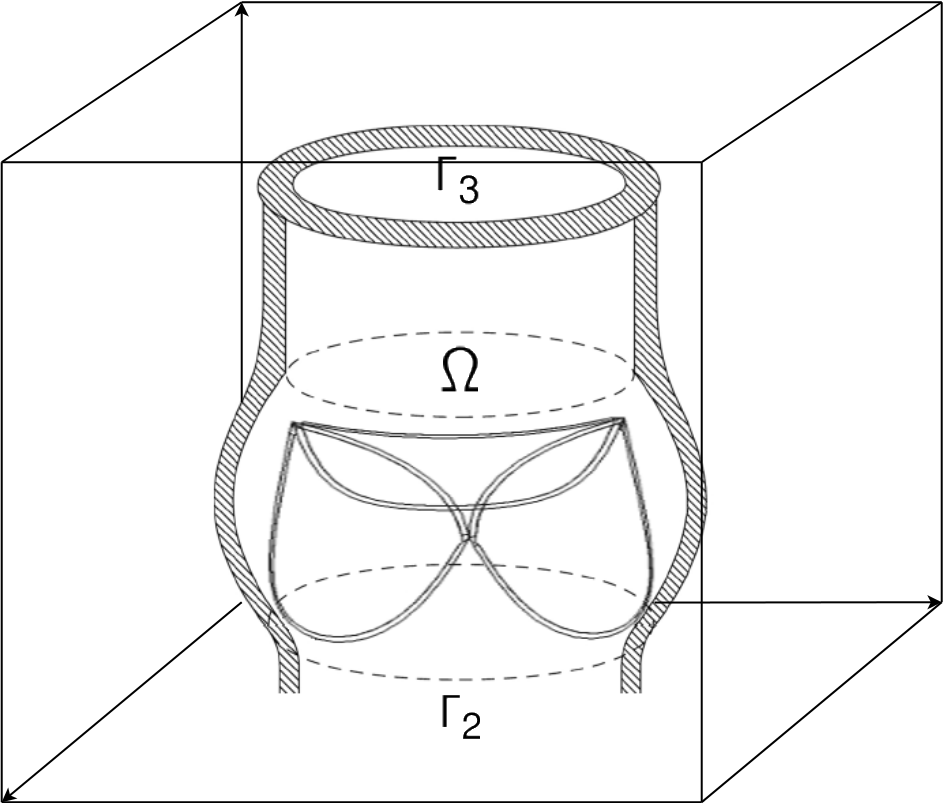
\includegraphics[width=8.5cm]{aorta_valve_scheme_framed.png}
    \end{center}
\end{frame}

% output data
\begin{frame}
\frametitle{Выходные данные}
В каждый момент времени модель полностью описывает:

\begin{itemize}
    \item[\MVRightarrow] Состояние жидкости, т.е. вектор скорости, давление
        внутри сосуда и распределение примеси, позволяя также определить
        интергальные характеристики, такие как расход жидкости.
    \item[\MVRightarrow] Состояние створок клапана - их форму и распределение
        напряжения деформации.
\end{itemize}

\end{frame}

% totals and examples
\begin{frame}
\frametitle{Примеры: распространение примеси}
    \begin{center}
        \vspace{-1.40mm}
        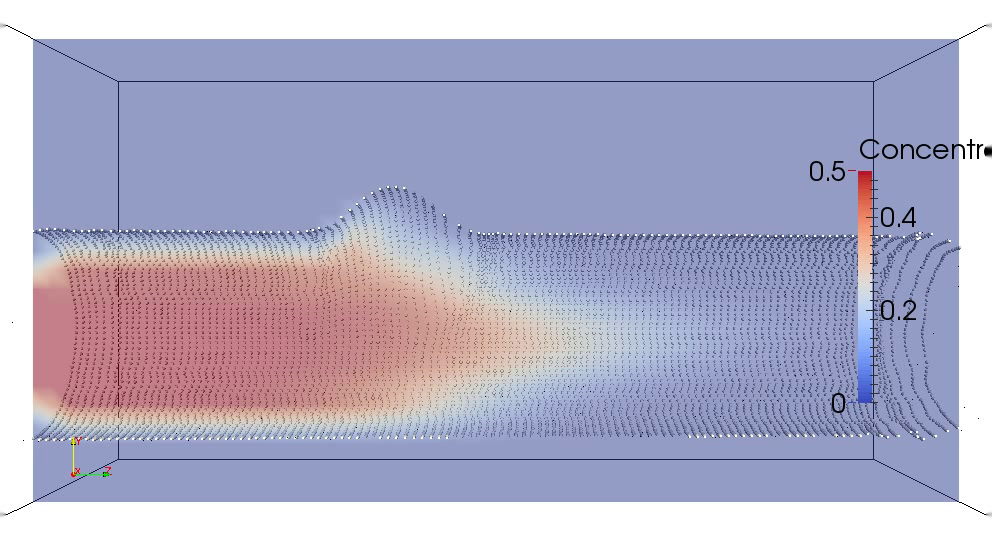
\includegraphics[width=7cm]{source_in_vessel_1.png}
        \vspace{0.40mm}
        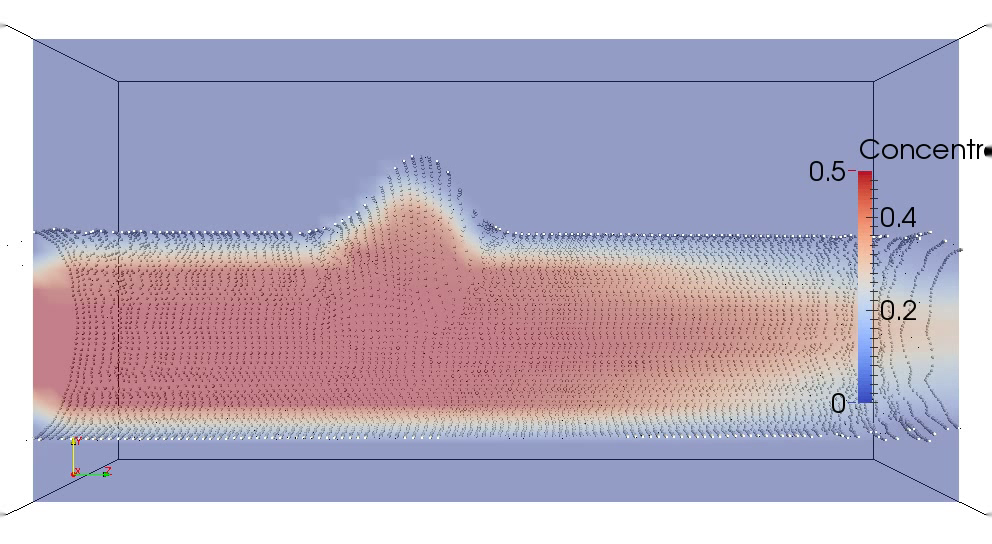
\includegraphics[width=7cm]{source_in_vessel_2.png}
    \end{center}
\end{frame}

% totals and examples
\begin{frame}
\frametitle{Примеры: размыв "тромба"}
    \begin{center}
        \vspace{-1.40mm}
        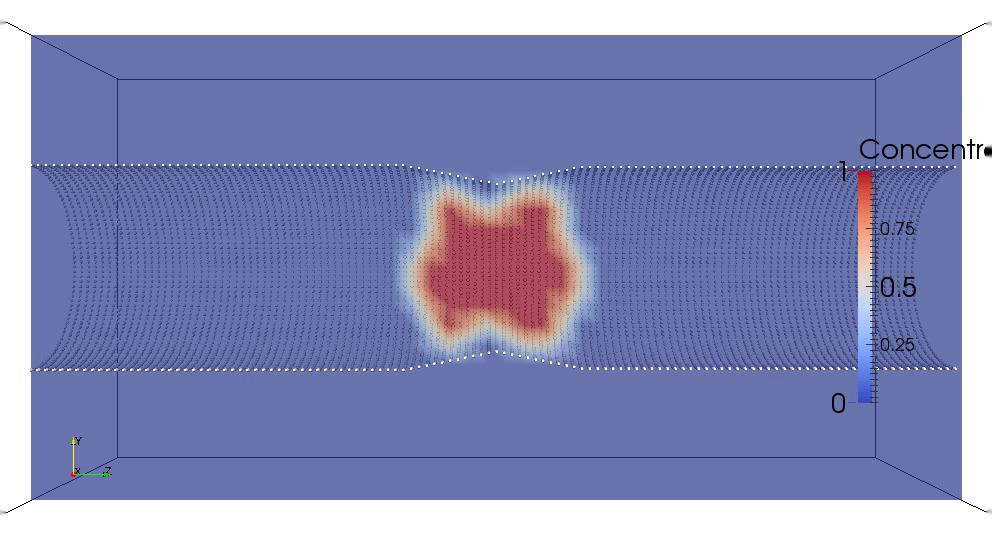
\includegraphics[width=7cm]{thrombus_in_vessel_1.png}
        \vspace{0.40mm}
        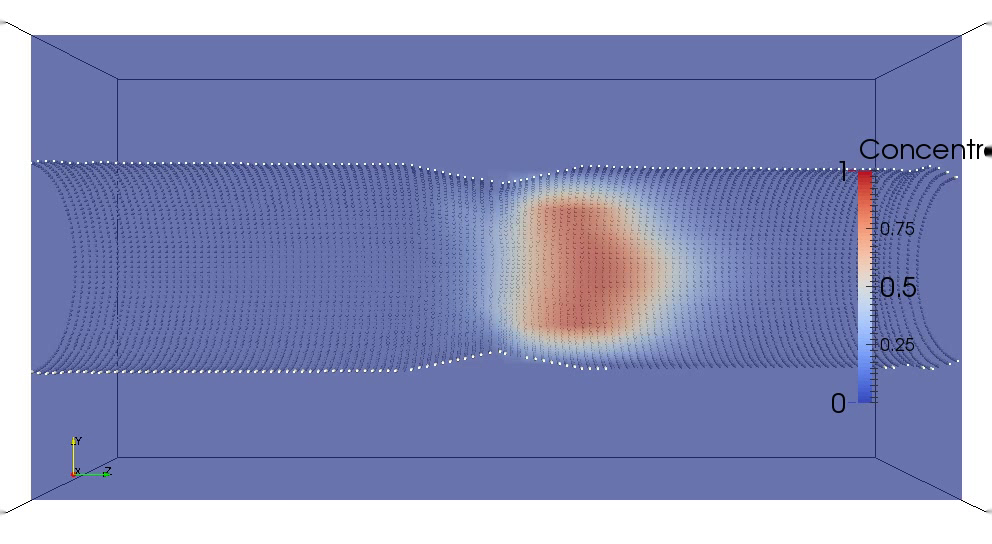
\includegraphics[width=7cm]{thrombus_in_vessel_2.png}
    \end{center}
\end{frame}

\begin{frame}
\frametitle{Примеры: движение клапана}
    \begin{center}
        \vspace{-1.40mm}
        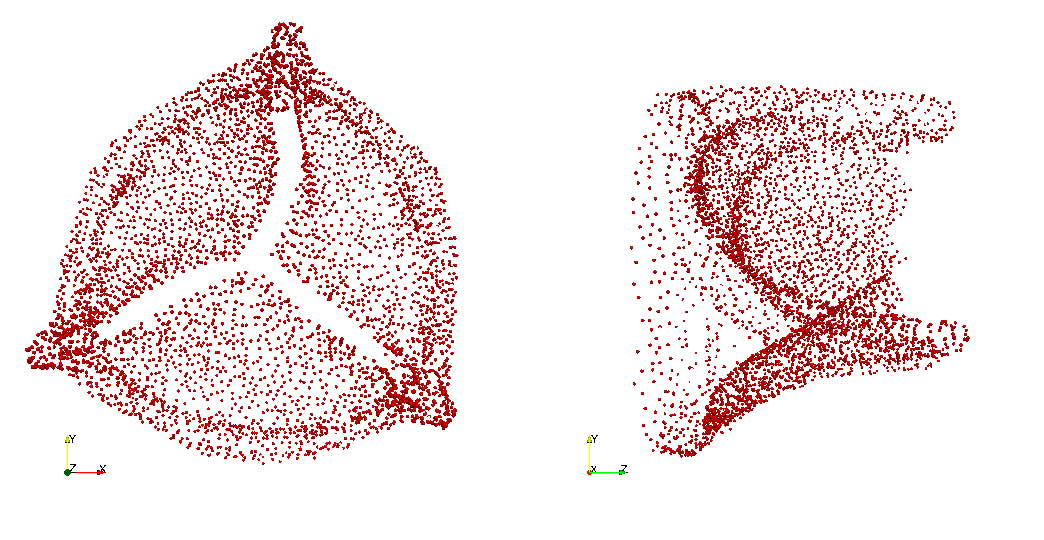
\includegraphics[width=7cm]{real_valve_1.png}
        \vspace{0.40mm}
        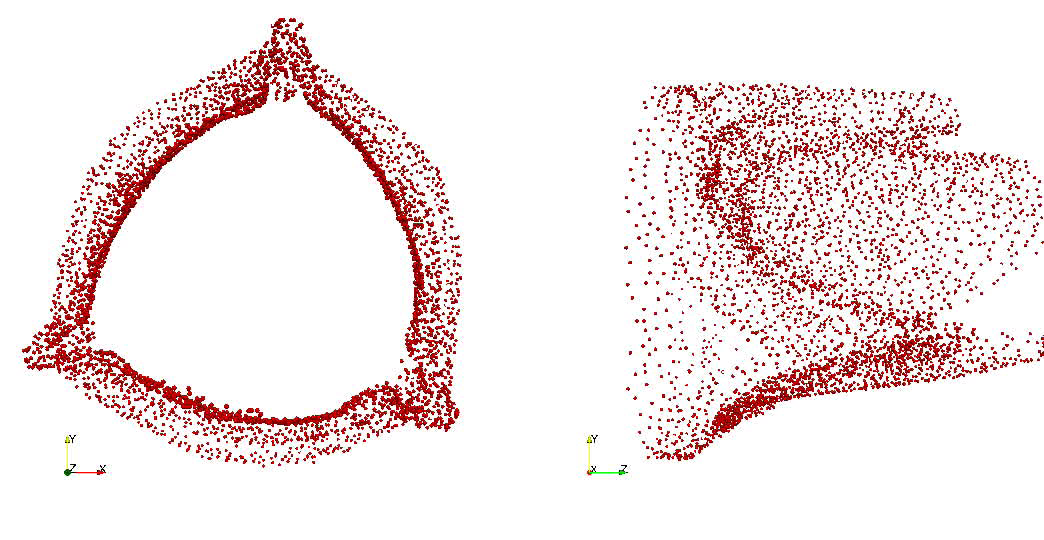
\includegraphics[width=7cm]{real_valve_2.png}
    \end{center}
\end{frame}

\begin{frame}
\frametitle{Примеры: поток внутри клапана}
    \begin{center}
        \vspace{-1.40mm}
        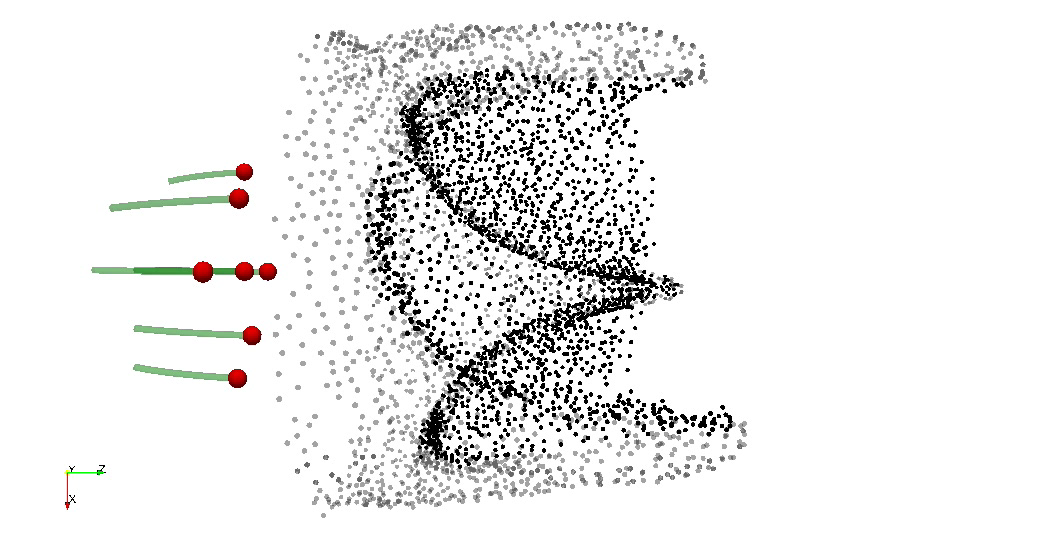
\includegraphics[width=7cm]{uniline_tracks_1.png}
        \vspace{0.40mm}
        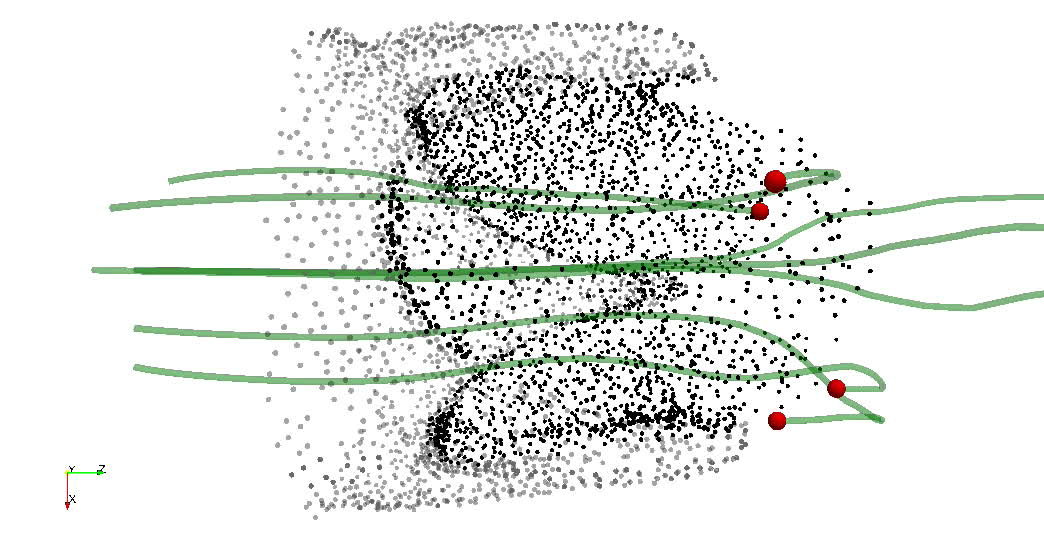
\includegraphics[width=7cm]{uniline_tracks_2.png}
    \end{center}
\end{frame}

\begin{frame}
\frametitle{Примеры: движение в примеси}
    \begin{center}
        \vspace{-1.40mm}
        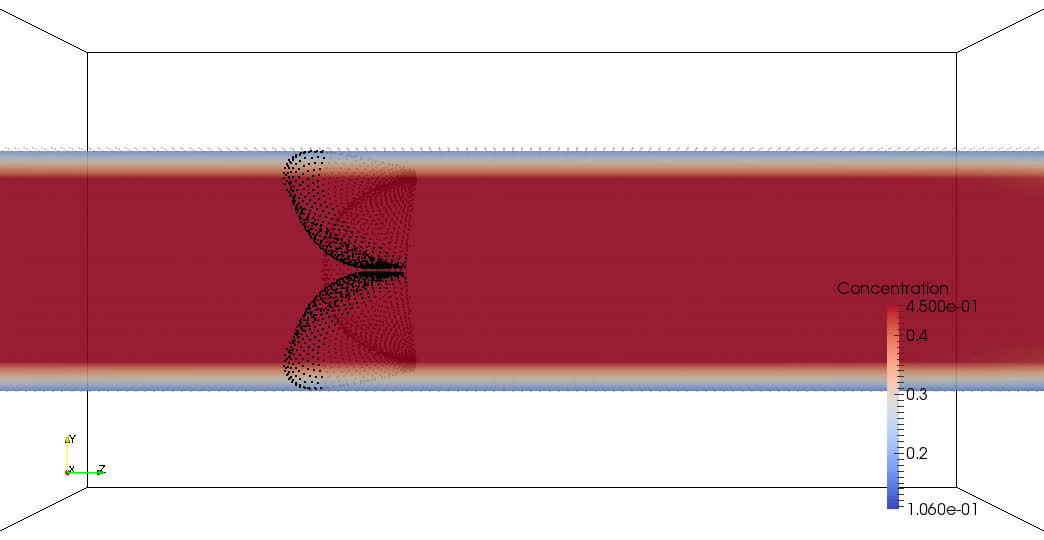
\includegraphics[width=7cm]{valve_in_mixture_1.png}
        \vspace{0.40mm}
        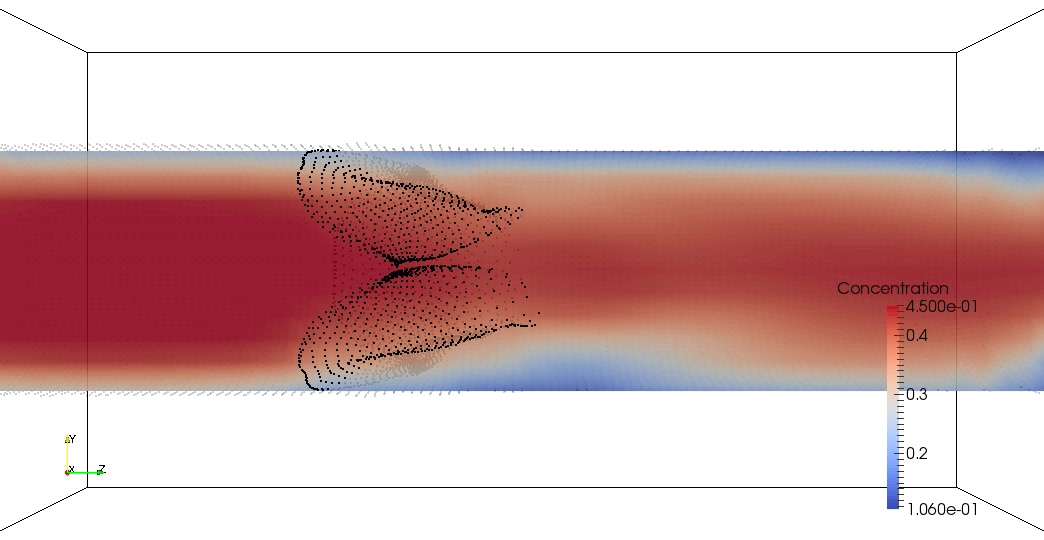
\includegraphics[width=7cm]{valve_in_mixture_2.png}
    \end{center}
\end{frame}

\begin{frame}
\frametitle{Напряжение}
    \begin{center}
        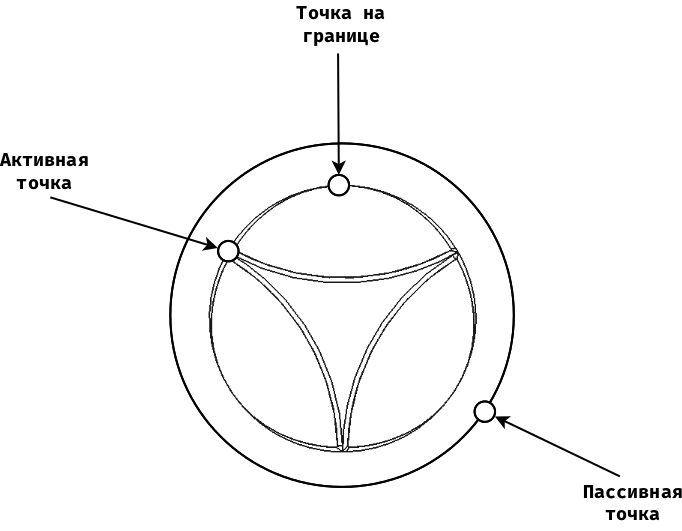
\includegraphics[width=9cm]{valve_points.png}
    \end{center}
\end{frame}

\begin{frame}
\frametitle{Напряжение}
    \begin{center}
        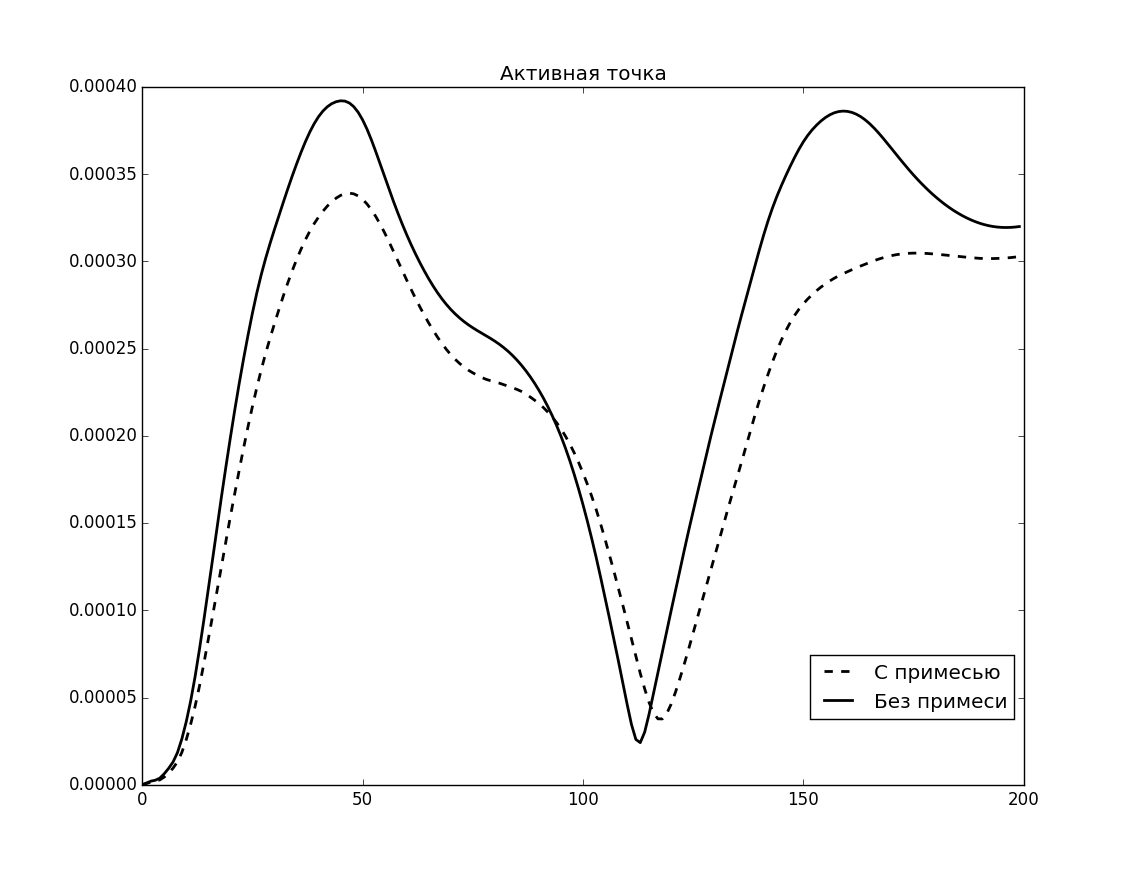
\includegraphics[width=10cm]{forces_active_point.png}
    \end{center}
\end{frame}

\begin{frame}
\frametitle{Напряжение}
    \begin{center}
        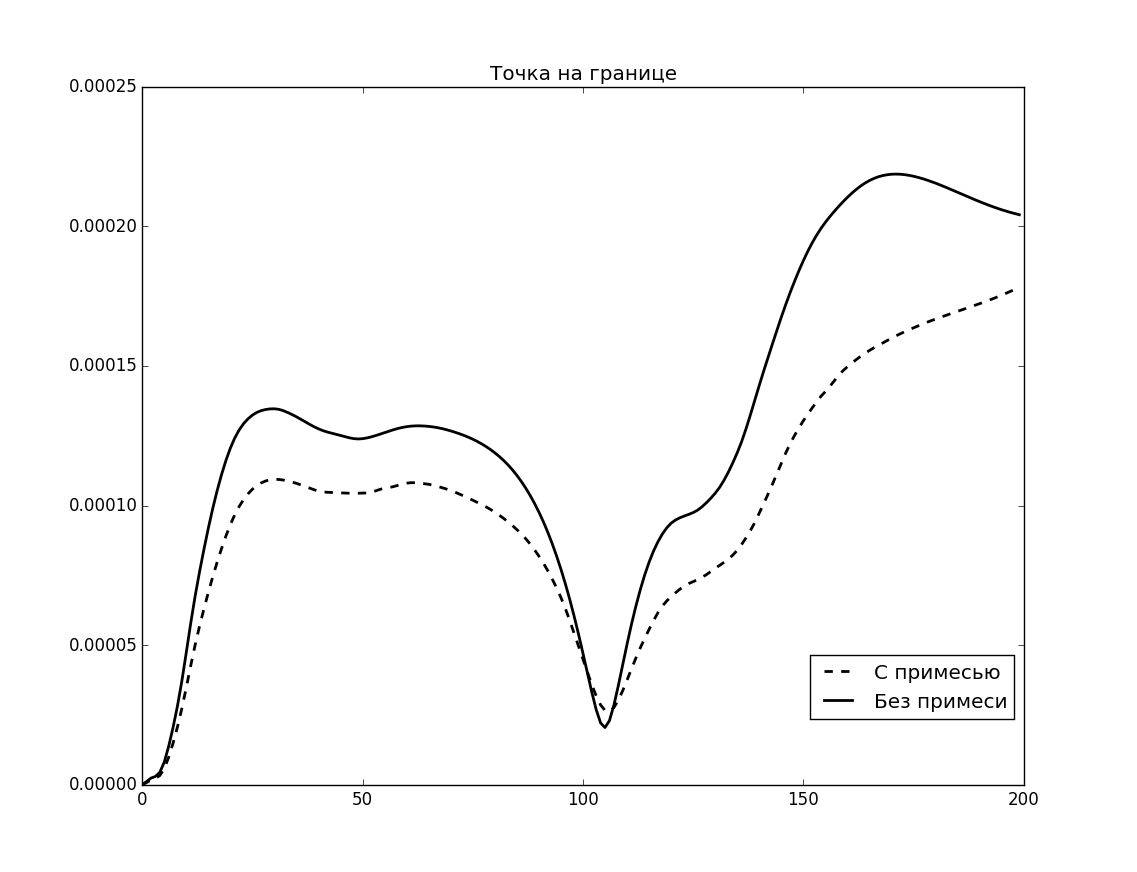
\includegraphics[width=10cm]{forces_boundary_point.png}
    \end{center}
\end{frame}

\begin{frame}
\frametitle{Напряжение}
    \begin{center}
        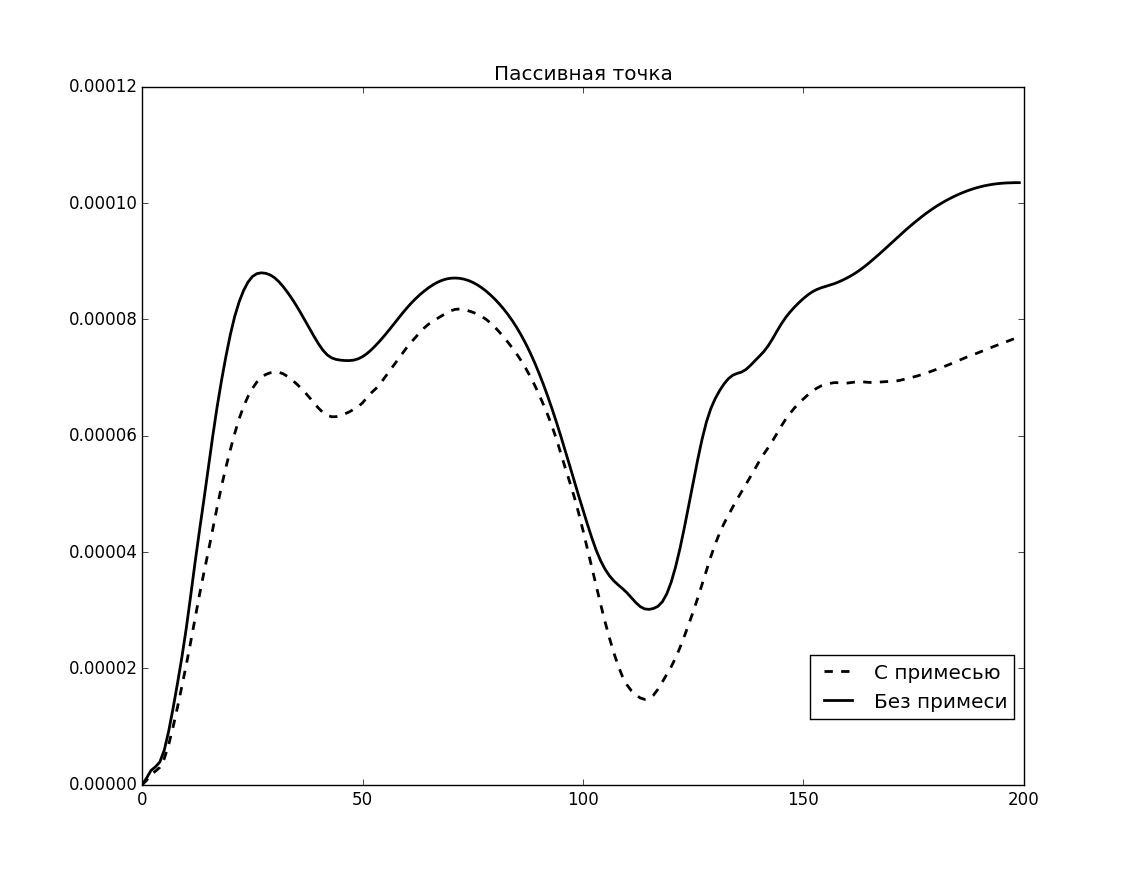
\includegraphics[width=10cm]{forces_passive_point.png}
    \end{center}
\end{frame}

\end{document}
